\documentclass[10pt,aspectratio=169]{beamer}

% Standalone presentation. Compile with pdfLaTeX.
\usetheme{default}
\usefonttheme{professionalfonts}
\usepackage[T1]{fontenc}
\usepackage{lmodern}
\usepackage{microtype}
\usepackage{tikz}
\usetikzlibrary{arrows.meta,positioning}

\definecolor{Navy}{HTML}{102A43}
\definecolor{Blue}{HTML}{246BCE}
\definecolor{Teal}{HTML}{0B8F87}
\definecolor{Sky}{HTML}{EAF3FF}
\definecolor{Mint}{HTML}{E8F6F4}
\definecolor{Ink}{HTML}{243B53}
\definecolor{Slate}{HTML}{627D98}
\definecolor{Rule}{HTML}{D9E2EC}
\definecolor{Paper}{HTML}{F8FAFC}
\definecolor{Amber}{HTML}{D97706}

\setbeamercolor{normal text}{fg=Ink,bg=white}
\setbeamercolor{structure}{fg=Blue}
\setbeamercolor{frametitle}{fg=Navy,bg=white}
\setbeamercolor{alerted text}{fg=Amber}
\setbeamerfont{title}{size=\fontsize{24}{28},series=\bfseries}
\setbeamerfont{subtitle}{size=\large}
\setbeamerfont{frametitle}{size=\Large,series=\bfseries}
\setbeamerfont{footline}{size=\tiny}
\setbeamersize{text margin left=0.65cm,text margin right=0.65cm}
\setbeamertemplate{navigation symbols}{}
\setbeamertemplate{itemize item}{\color{Teal}$\blacktriangleright$}

\setbeamertemplate{frametitle}{%
  \nointerlineskip
  \vspace{0.42cm}
  \insertframetitle\par
  \vspace{0.12cm}
  {\color{Rule}\rule{\textwidth}{0.8pt}}
}

\setbeamertemplate{footline}{%
  \leavevmode
  \hbox{%
    \begin{beamercolorbox}[wd=.78\paperwidth,ht=2.7ex,dp=1.2ex,leftskip=.65cm]{normal text}%
      \color{Slate}\usebeamerfont{footline}ECON 5166 \enspace|\enspace Group 2
    \end{beamercolorbox}%
    \begin{beamercolorbox}[wd=.22\paperwidth,ht=2.7ex,dp=1.2ex,rightskip=.65cm plus1fil]{normal text}%
      \hfill\color{Slate}\usebeamerfont{footline}\insertframenumber\,/\,\inserttotalframenumber
    \end{beamercolorbox}%
  }
}

\newcommand{\eyebrow}[1]{%
  {\color{Teal}\bfseries\fontsize{8.5}{10}\selectfont\MakeUppercase{#1}}}

\newcommand{\statcard}[3]{%
  \begin{minipage}[t]{0.30\textwidth}
    \begin{tikzpicture}
      \node[rounded corners=4pt,fill=#1,inner sep=8pt,
            text width=0.88\linewidth,minimum height=1.45cm,align=left] {
        {\color{Navy}\fontsize{19}{21}\selectfont\bfseries #2}\par
        \vspace{2pt}{\color{Slate}\fontsize{8.5}{10}\selectfont #3}
      };
    \end{tikzpicture}
  \end{minipage}}

\newcommand{\outputcard}[3]{%
  \begin{minipage}[t]{0.305\textwidth}
    \begin{tikzpicture}
      \node[rounded corners=4pt,draw=Rule,line width=.8pt,fill=white,
            inner sep=8pt,text width=0.88\linewidth,minimum height=2.35cm,
            align=left] {
        {\color{Teal}\bfseries #1}\par\vspace{4pt}
        {\color{Navy}\bfseries #2}\par\vspace{3pt}
        {\color{Slate}\scriptsize #3}
      };
    \end{tikzpicture}
  \end{minipage}}

\title{Understanding Nighttime Traffic Crashes in Taipei}
\subtitle{Road-environment clusters, lighting conditions, and crash severity}
\author{Tzu-Chuan Hsieh \quad Yi-Han Tseng \quad Ming-Han Chan}
\institute{National Taiwan University}
\date{October 2026}

\begin{document}

\begin{frame}[plain]
% message: Introduce the study as a three-minute proposal for identifying actionable nighttime crash contexts.
% presenter notes (0:00--0:15):
% - Introduce Group 2 and preview the talk: why, how, and expected results.
\begin{tikzpicture}[remember picture,overlay]
  \fill[Navy] (current page.north west)
    rectangle ([xshift=4.75cm]current page.south west);
  \fill[Teal] ([xshift=4.75cm]current page.north west)
    rectangle ([xshift=4.86cm]current page.south west);
\end{tikzpicture}

\begin{columns}[onlytextwidth,c]
  \begin{column}{0.26\textwidth}
    \color{white}
    {\bfseries\fontsize{8.5}{10}\selectfont RESEARCH PROPOSAL}\par
    \vspace{0.35cm}
    {\fontsize{25}{28}\selectfont\bfseries 3-MINUTE\\PRESENTATION}\par
    \vspace{0.55cm}
    {\small ECON 5166\\Group 2}
  \end{column}
  \begin{column}{0.68\textwidth}
    {\color{Navy}\usebeamerfont{title}\inserttitle}\par
    \vspace{0.25cm}
    {\color{Teal}\usebeamerfont{subtitle}\insertsubtitle}\par
    \vspace{0.7cm}
    {\color{Ink}\small\insertauthor}\par
    \vspace{0.14cm}
    {\color{Slate}\small\insertinstitute \enspace|\enspace \insertdate}
  \end{column}
\end{columns}
\end{frame}

% -----------------

\begin{frame}{Why This Study?}
% message: Citywide averages can hide meaningful differences among nighttime crash contexts.
% presenter notes (0:15--1:00):
% - Contrast intersections, arterial roads, alleys, and peripheral roads.
% - Treat the figures as preliminary descriptive statistics, not clustering results.
% - State the research question at the bottom.

\eyebrow{The problem}\par
\vspace{0.18cm}
{\large\bfseries\color{Navy}
Nighttime crashes occur in different road environments---but averages treat them as one.}

\vspace{0.38cm}
\begin{center}
  \statcard{Sky}{\(\sim\)6,795}{nighttime injury crashes in Taipei, 2025}
  \hfill
  \statcard{Mint}{363}{cases with lights off or malfunctioning}
  \hfill
  \statcard{Sky}{97}{cases recorded on unlit roads}
\end{center}

\vspace{0.32cm}
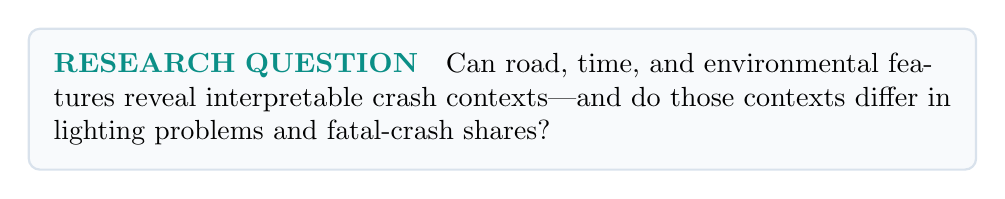
\begin{tikzpicture}
  \node[rounded corners=4pt,fill=Paper,draw=Rule,line width=.8pt,
        inner sep=9pt,text width=.94\textwidth,align=left] {
    {\color{Teal}\bfseries RESEARCH QUESTION}\quad
    Can road, time, and environmental features reveal interpretable crash contexts---and do
    those contexts differ in lighting problems and fatal-crash shares?
  };
\end{tikzpicture}

\vfill
{\color{Slate}\tiny Note: counts are preliminary descriptive statistics, not clustering results.}
\end{frame}

% -----------------

\begin{frame}{How Will We Study It?}
% message: Separate context formation from outcome comparison to avoid defining clusters by the results.
% presenter notes (1:00--2:10):
% - Define nighttime from sunset to the next sunrise.
% - Explain feature processing, PCA, hierarchical guidance, and k-means from K=2 to K=6.
% - Emphasize that lighting, deaths, and injuries are held out of clustering.

\eyebrow{Analysis design}\par
\vspace{0.28cm}

\centering
\begin{tikzpicture}[
  step/.style={rounded corners=4pt,draw=Rule,line width=.8pt,fill=white,
               text width=2.58cm,minimum height=2.15cm,inner sep=7pt,align=left},
  flow/.style={-{Latex[length=2.3mm]},line width=1.2pt,draw=Teal}
]
  \node[step] (s1) {
    {\color{Teal}\bfseries 01}\par\vspace{3pt}
    {\color{Navy}\bfseries Define the sample}\par\vspace{3pt}
    {\color{Slate}\scriptsize 2025 injury crashes; sunset to next sunrise}
  };
  \node[step,right=0.38cm of s1] (s2) {
    {\color{Teal}\bfseries 02}\par\vspace{3pt}
    {\color{Navy}\bfseries Build features}\par\vspace{3pt}
    {\color{Slate}\scriptsize Time, speed, weather, road type, and position}
  };
  \node[step,right=0.38cm of s2] (s3) {
    {\color{Teal}\bfseries 03}\par\vspace{3pt}
    {\color{Navy}\bfseries Reduce + cluster}\par\vspace{3pt}
    {\color{Slate}\scriptsize PCA, hierarchical guidance, k-means \(K=2\)--\(6\)}
  };
  \node[step,right=0.38cm of s3] (s4) {
    {\color{Teal}\bfseries 04}\par\vspace{3pt}
    {\color{Navy}\bfseries Compare outcomes}\par\vspace{3pt}
    {\color{Slate}\scriptsize Lighting, fatalities, injuries, and geography}
  };
  \draw[flow] (s1) -- (s2);
  \draw[flow] (s2) -- (s3);
  \draw[flow] (s3) -- (s4);
\end{tikzpicture}

\vspace{0.48cm}
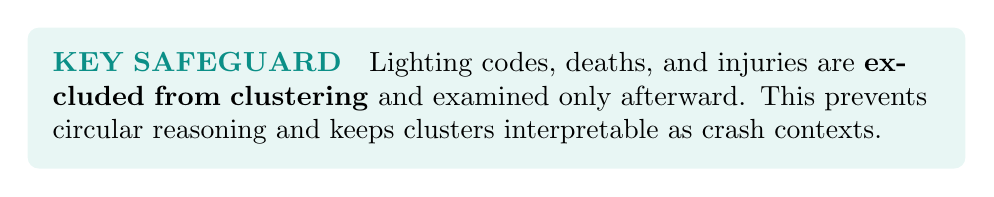
\begin{tikzpicture}
  \node[rounded corners=4pt,fill=Mint,inner sep=9pt,
        text width=.93\textwidth,align=left] {
    {\color{Teal}\bfseries KEY SAFEGUARD}\quad
    Lighting codes, deaths, and injuries are \textbf{excluded from clustering} and examined only afterward.
    This prevents circular reasoning and keeps clusters interpretable as crash contexts.
  };
\end{tikzpicture}

\vfill
{\color{Slate}\scriptsize Cluster selection combines elbow and silhouette evidence, stability, cluster size, and substantive interpretability.}
\end{frame}

% -----------------

\begin{frame}{What Do We Expect to Deliver?}
% message: Convert interpretable crash contexts into defensible inspection priorities without making causal claims.
% presenter notes (2:10--3:00):
% - Name clusters only after examining their observed profiles.
% - Explain the priority matrix: crash count multiplied by lighting-problem share.
% - Close with the policy value and the non-causal boundary.

\eyebrow{Expected results}\par
\vspace{0.3cm}

\begin{center}
  \outputcard{01}{Crash contexts}{Stable, interpretable clusters named from observed road, time, and environmental profiles.}
  \hfill
  \outputcard{02}{Outcome differences}{Cluster-level lighting conditions, fatal-crash shares, and 95\% confidence intervals.}
  \hfill
  \outputcard{03}{Inspection priorities}{A matrix combining crash volume and lighting-problem share to identify cases worth checking first.}
\end{center}

\vspace{0.42cm}
\begin{columns}[onlytextwidth,T]
  \begin{column}{0.63\textwidth}
    {\color{Navy}\large\bfseries Decision value}\par
    \vspace{0.12cm}
    {\small Help the city prioritize field checks, verify streetlight status, and target follow-up data collection on illumination, traffic volume, and road design.}
  \end{column}
  \begin{column}{0.33\textwidth}
    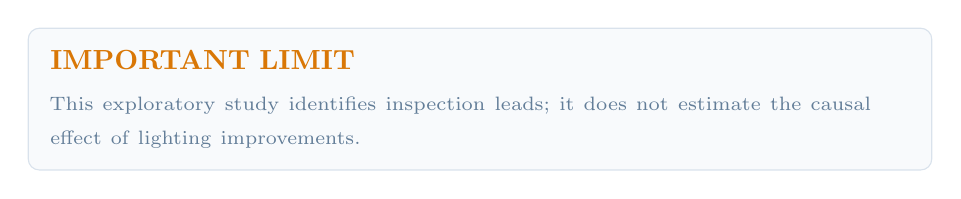
\begin{tikzpicture}
      \node[rounded corners=4pt,fill=Paper,draw=Rule,inner sep=8pt,
            text width=.9\linewidth,align=left] {
        {\color{Amber}\bfseries IMPORTANT LIMIT}\par\vspace{3pt}
        {\color{Slate}\scriptsize This exploratory study identifies inspection leads; it does not estimate the causal effect of lighting improvements.}
      };
    \end{tikzpicture}
  \end{column}
\end{columns}

\vfill
\centering
{\color{Teal}\bfseries Better segmentation \(\rightarrow\) more focused inspection \(\rightarrow\) better evidence for future action}
\end{frame}

\end{document}
